\chapter{Introduction}
\label{intro}

Background Info on white dwarfs and exoplanetary systems:
\section{Exoplanets}
Rise of the field, importance for understanding diversity of planetary systems
Context for pulsar planet as first exoplanet detection, lead in to post-stellar evolution objects. 

Work notes: mostly text, lit review.
\section{Transits}
Introduction to transit method (not very long)
Discussion of why WDs are favorable for transit detections: comparison figure of lightcurves for Earth transiting Sun vs WD

Work notes: mostly text, lit review. Make one figure.
\section{WD Transit Motivation}
Debris disks+ Polluted WDs: frequency, sinking timescales, overview of past work as motivation for transit studies. We know there are planetary remnants there.
K2 mission and guest proposals.

Work notes: Text. lit review +  go over other K2 guest proposals.
\section{WD1145 Detection}
Details regarding detection and a little information about followup photometry (more in Chapter \ref{chapter_photo}). 
Then \cite{Xu2016} detection of circumstellar absorption, leads into discussion of next section.

Work notes: Do some work with available K2 photometry papers to find the best way to summarize object's behavior. Pick out a stellar line to show CS absorption clearly: strong, isolated, preferably from Xu data to show blue and red edges. Or a more large-scale view like \cite{Xu2016} Fig 1a/b?
\section{Significance of WD1145} 
Explanation of lack of knowledge of planetary interiors: RV + transit constrain Mass/Radius $\implies \rho$, transit and eclispse spectroscopy give atmospheric info, but now we use WD as our mass spectrometer to get information about planetary interior. To give context, list some other known disintegrating planetary systems or other ways we've constrained composition (find the iron exo-Mercury that was identified because its orbital period requires that composition to avoid the disintegration we see here)

Work notes: lots of lit review (bring in work with disks, but not too much because that will get discussed more in Chapter \ref{chapter_spectra})


\section{Figure+Citation}

Look figure + citation: \citep[e.g.,][see Fig. \ref{PrettyPic}]{Vanderburg2015}. 

\begin{figure}
\centering
\scalebox{0.45}{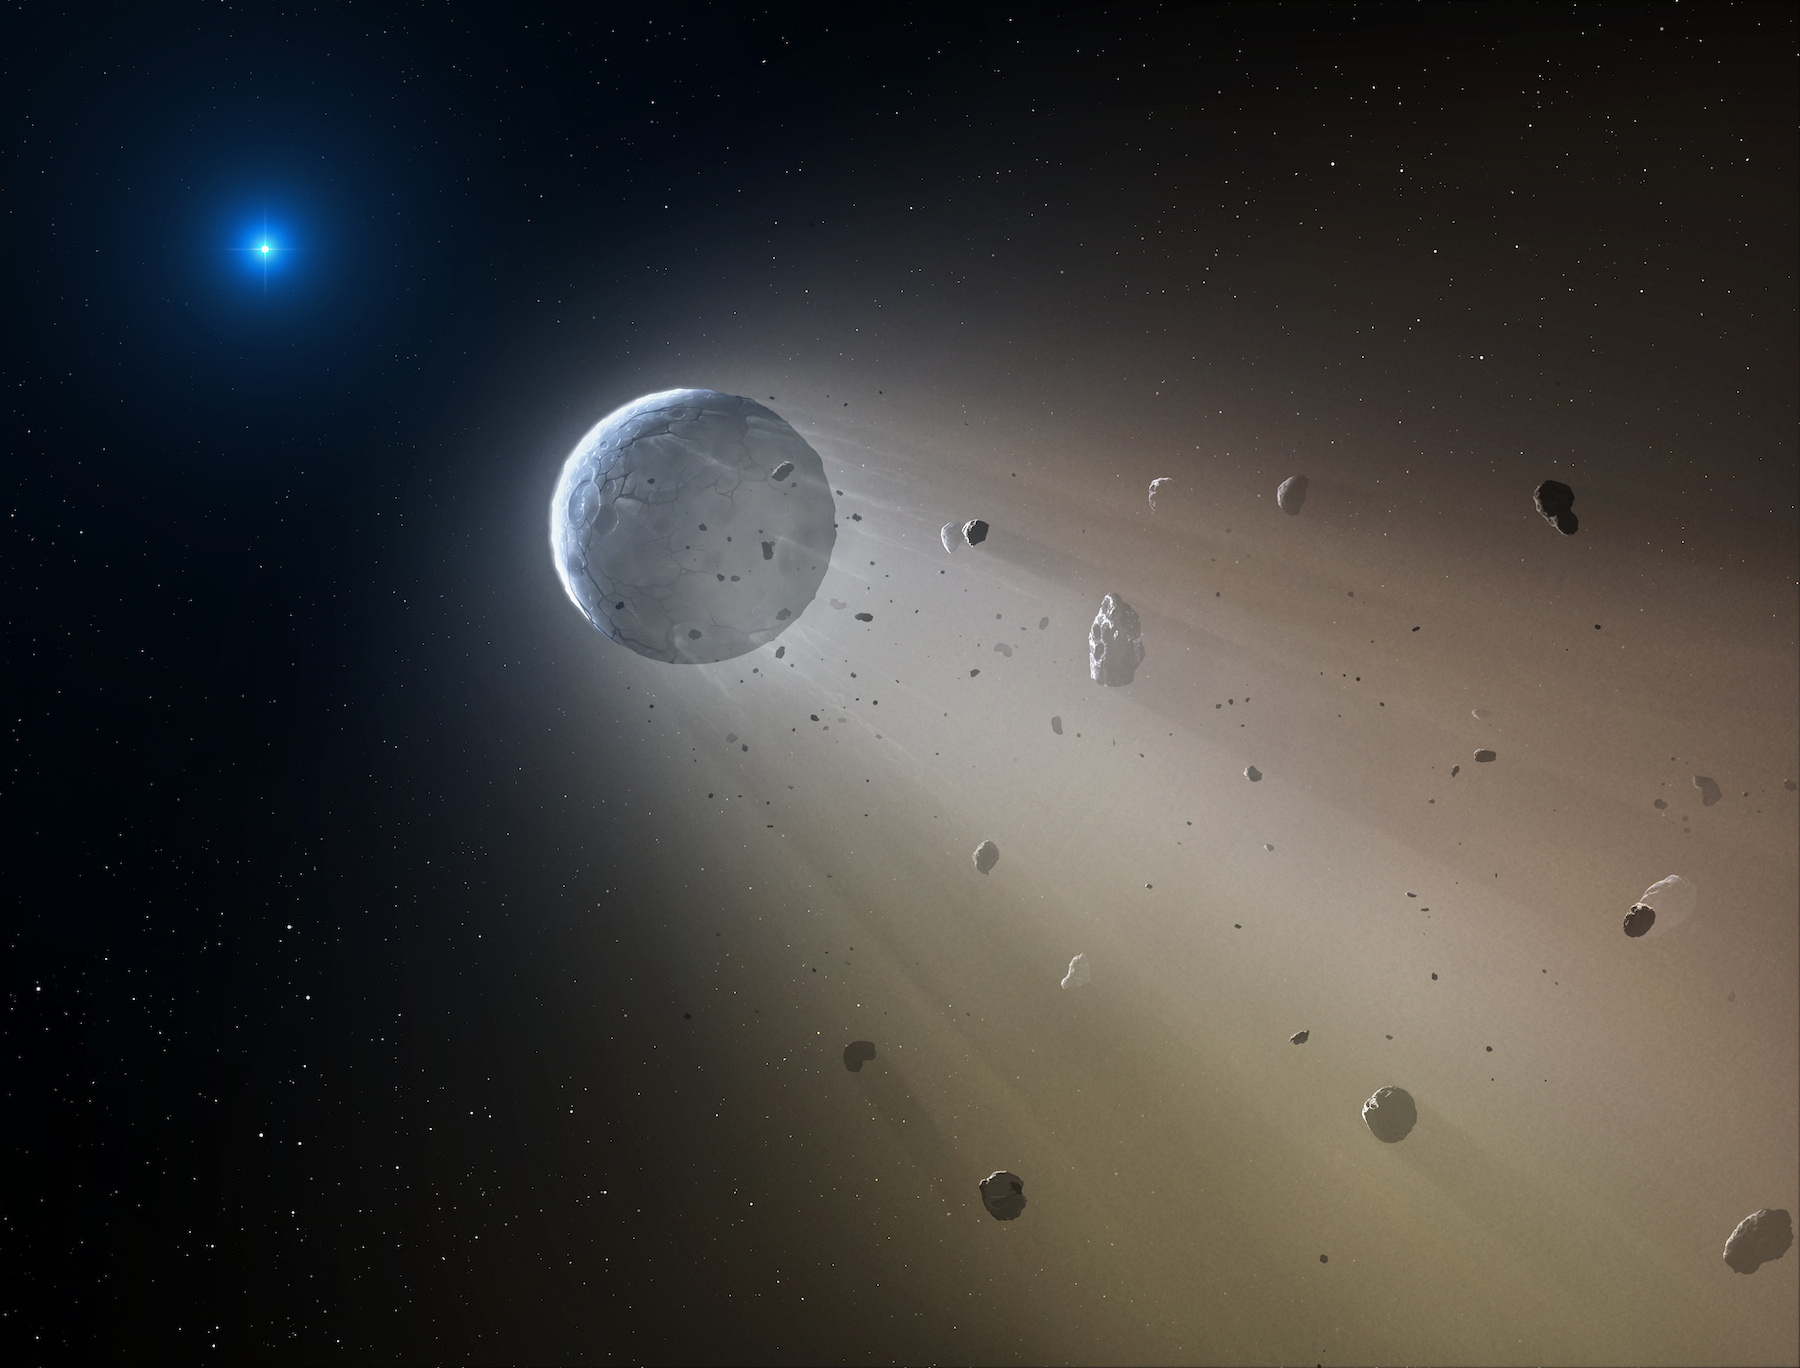
\includegraphics{Figures/PrettyPic.png}}
\caption{The artist rendition of WD1145+017 \citep[from][]{Vanderburg2015}.}
\label{PrettyPic}
\end{figure}

%\ifthenelse{\isodd{\thepage}}{\clearemptydoublepage}{}